\documentclass[../main.tex]{subfiles}

\begin{document}

\theoremstyle{definition}
\newtheorem{Def}{Définition}

\theoremstyle{plain}
\newtheorem{Conj}{Conjecture}

    \label{sec:test2}
    Dans cette section, nous allons vérifier si des conjectures sur les nombres premiers peuvent s'appliquer aux ensembles aléatoires créés à la section \ref{sec:sec1}. Ainsi, on sera en mesure d'estimer si la véracité d'une conjecture est susceptible de tenir grâce à la répartition des nombres premiers plutôt qu'à leur propriété d'être premier. 
 
 \subsection{Les nombres premiers jumeaux} 
 	La première conjecture que nous allons analyser, et sans doute la plus célèbre, est la conjecture des nombres premiers jumeaux.
	\begin{Def}
	Soient $a$, $b \in \mathbb{N} $, $ a < b$, on dit que $a$ et $b$ sont jumeaux si $ a + 2 = b $.
	\end{Def}  
	
	\begin{Conj}
	Il y a une infinité de nombres premiers jumeaux.
	\end{Conj}
	
	Ces dernières années, il y'a eu de grosses avancées dans la démonstration de la conjecture. Ainsi, pour tout $ m \geqslant 1$, soit $H_{m} := $ $\liminf_{n \rightarrow \infty}  (p_{n+m} - p_{n})$, où $p_{n}$ dénote le n-ième nombre premier. La conjecture des nombres premiers jumeaux est donc équivalente à $H_{1} = 2$. En 2013, le mathématicien chinois Zhang Yitang est le premier à trouver une borne supérieure finie pour $H_{1}$, il a démontré que $H_{1} \leqslant 70\, 000\, 000$. Suite à la publication de Zhang Yitang, de nombreux mathématiciens se sont mis en quête de réduire la borne supérieure de $H_{1}$. En optimisant les résultats de Zhang Yitang et grâce à d'autres méthodes ils ont pu montrer que $H_{1} \leqslant 246$.
	
	Afin de tester la conjecture sur les ensembles aléatoires, nous avons tracé un graphe (figure \ref{im:image4}), où pour chaque ensembles aléatoires et l'ensemble des nombres premiers (jusqu'à $10^{7}$) on trace une fonction qui compte le nombre de jumeaux.
\begin{figure}[htbp]
	\centerline{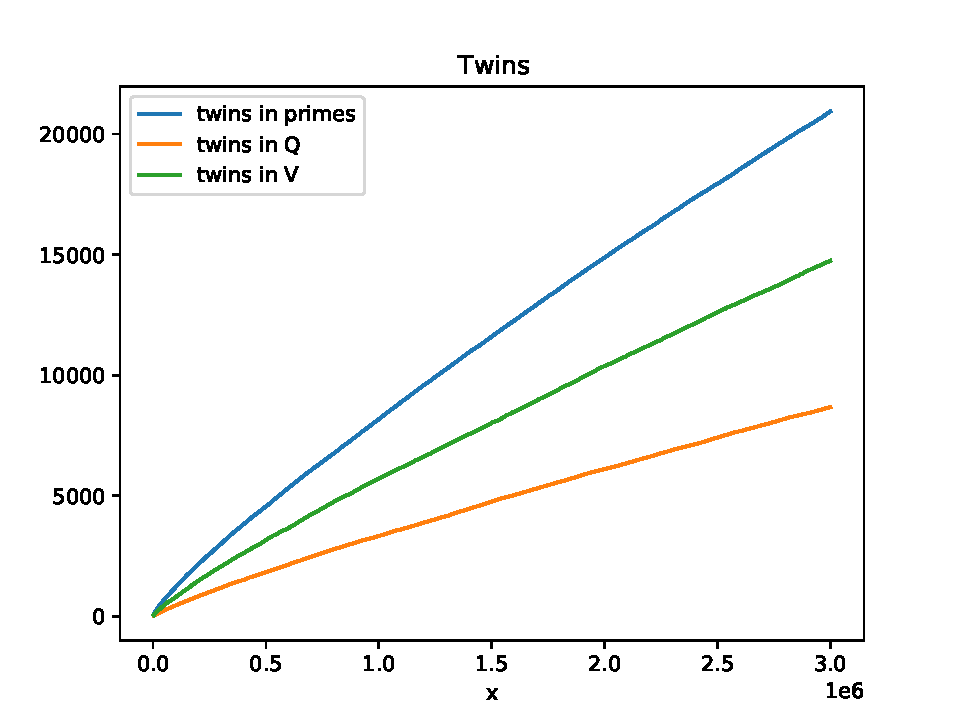
\includegraphics[width = \textwidth]{twins.pdf}}
\caption{Nombre de jumeaux dans chaque ensemble }
	\label{im:image4}
\end{figure}
 Nous pouvons faire les observations suivantes : 
 	\begin{itemize}
	\item Pour chaque type d'ensemble (selon l'approche utilisée), on constate, logiquement, que le nombre de jumeaux est plus ou moins le double pour les ensembles impairs.
	\item Il y'a plus de jumeaux dans les ensembles $R$ que dans les ensembles $Q$ ce qui peut s'expliquer par le fait qu'ils ont plus d'éléments que les ensembles $Q$.
	\item De manière générale, toutes les courbes sont croissantes, ce qui indiquerait, autant pour les nombres premiers que pour les ensembles aléatoires, que le nombre de jumeaux tend vers l'infini. 
	\end{itemize}
	
	De plus, ce graphe éveille une idée intéressante. Si on désigne par $f$ la fonction qui compte le nombre de jumeaux dans l'ensemble des nombres premiers et par $g$ celle qui compte les jumeaux dans un ensemble aléatoire et qu'on parvient à montrer que $f$ et $g$ sont semblables (sous-entendu qu'elles le sont), alors $\lim\limits_{x \rightarrow \infty} g(x) = \infty \Rightarrow \lim\limits_{x \rightarrow \infty} f(x) = \infty $. Ce qui démontrerait la conjecture des nombres premiers jumeaux. Pour ce faire une idée d'une éventuelle équivalence entre $f$ et $g$, voici le graphe (figure \ref{im:image6}) de $\frac{f(x)}{g(x)}$, où $g$ est appliquée à un ensemble impair $Q$ choisi arbitrairement. 
	
\begin{figure}[htbp]
	\centerline{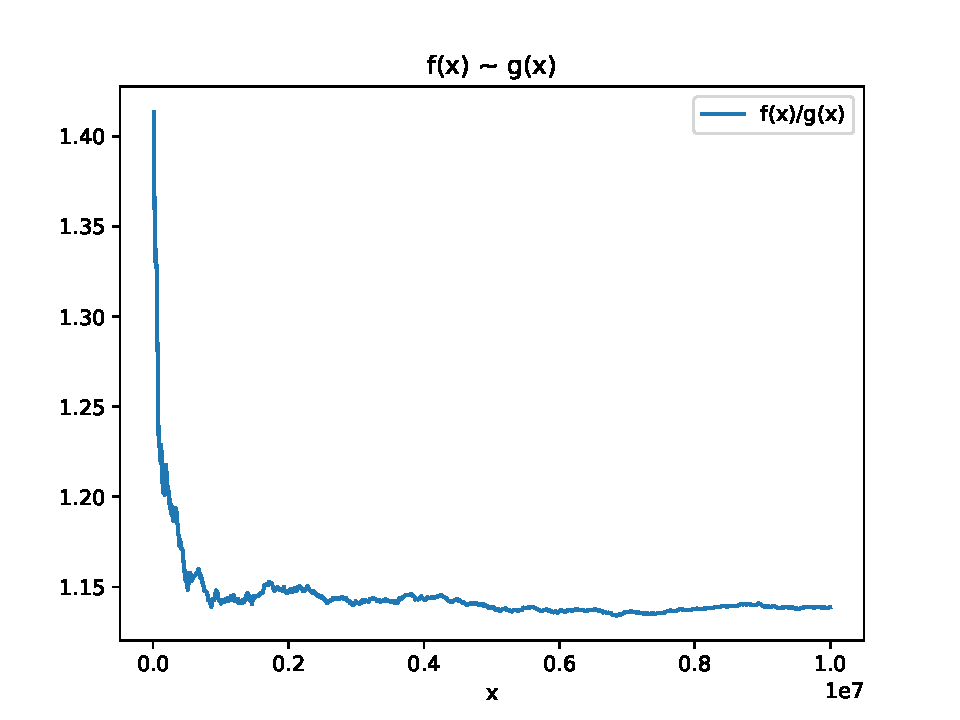
\includegraphics[width = \textwidth]{ecarts_count_twins.pdf}}
\caption{$\frac{f(x)}{g(x)}$}
	\label{im:image6}
\end{figure}

\clearpage
\end{document}




